
\documentclass[10pt,onecolumn,letterpaper]{article}

\usepackage{iccv}
\usepackage{times}
\usepackage{epsfig}
\usepackage{graphicx}
\usepackage{amsmath}
\usepackage{amssymb}
\usepackage[numbers,sort]{natbib}

\usepackage{subfigure}
\usepackage{upgreek}
\usepackage{multirow}
\usepackage{color}
\usepackage{bm}
\DeclareMathOperator*{\argmin}{arg\,min}
\usepackage{arydshln}
\usepackage{latexsym}


\usepackage{amsthm}
\newtheorem{theorem}{Theorem}
\newtheorem{lemma}[theorem]{Lemma}
\newtheorem{conj}[theorem]{Conjecture}


% Include other packages here, before hyperref.

% If you comment hyperref and then uncomment it, you should delete
% egpaper.aux before re-running latex.  (Or just hit 'q' on the first latex
% run, let it finish, and you should be clear).
\usepackage[pagebackref=true,breaklinks=true,letterpaper=true,colorlinks,bookmarks=false]{hyperref}

% \iccvfinalcopy % *** Uncomment this line for the final submission

\def\iccvPaperID{572} % *** Enter the ICCV Paper ID here
\def\httilde{\mbox{\tt\raisebox{-.5ex}{\symbol{126}}}}

% Pages are numbered in submission mode, and unnumbered in camera-ready
\ificcvfinal\pagestyle{empty}\fi
\begin{document}

%%%%%%%%% TITLE
\title{Supplementary File to ``Multi-channel Weighted Nuclear Norm Minimization for Real Color Image Denoising''}

\author{First Author\\
Institution1\\
Institution1 address\\
{\tt\small firstauthor@i1.org}
% For a paper whose authors are all at the same institution,
% omit the following lines up until the closing ``}''.
% Additional authors and addresses can be added with ``\and'',
% just like the second author.
% To save space, use either the email address or home page, not both
\and
Second Author\\
Institution2\\
First line of institution2 address\\
{\tt\small secondauthor@i2.org}
}

\maketitle
%\thispagestyle{empty}


In this supplementary file, we provide:\vspace{-2mm}
\begin{enumerate}
\item The proof of the Theorem 1 in the main paper.
\vspace{-2mm}
\item More denoising results on the 24 high quality images from the Kodak PhotoCD dataset.\vspace{-2mm}
\item More visual comparisons of denoised images by different methods on the real noisy images of the dataset \cite{ncwebsite}. \vspace{-2mm}
\item More visual comparisons of denoised images by different methods on the real noisy images of the dataset \cite{crosschannel2016}.
\end{enumerate}


\section{Proof of Theorem 1.}
\begin{theorem}
Assume that the weights in $\bm{w}$ are in a non-descending order, the sequence $\{\mathbf{X}_{k}\}$, $\{\mathbf{Z}_{k}\}$, and $\{\mathbf{A}_{k}\}$ generated in Algorithm 1 satisfy:
\begin{equation}
(a) \lim_{k \to \infty} \|\mathbf{X}_{k+1}-\mathbf{Z}_{k+1}\|_{F}=0;
\quad
(b) \lim_{k \to \infty} \|\mathbf{X}_{k+1}-\mathbf{X}_{k}\|_{F}=0;
\quad
(c) \lim_{k \to \infty} \|\mathbf{Z}_{k+1}-\mathbf{Z}_{k}\|_{F}=0.
\end{equation}
\end{theorem}
\begin{proof}
1.\ Firstly, we prove that the sequence $\{\mathbf{A}_{k}\}$ generated by Algorithm 1 is upper bounded.
Let $\mathbf{X}_{k+1}+\rho_{k}^{-1}\mathbf{A}_{k}
=
\mathbf{U}_{k}\mathbf{\Sigma}_{k}\mathbf{V}_{k}^{\top}$
be its singular value decomposition (SVD) \cite{eckart1936approximation} in the $(k+1)$-th iteration. According to Corollary 1 of \cite{wnnmijcv}, we can have the SVD of $\mathbf{Z}_{k+1}$ as $\mathbf{Z}_{k+1}=\mathbf{U}_{k}\hat{\mathbf{\Sigma}}_{k}\mathbf{V}_{k}^{\top}=\mathbf{U}_{k}\mathcal{S}_{\frac{\bm{w}}{\rho_{k}}}(\mathbf{\Sigma}_{k})\mathbf{V}_{k}^{\top}$. 
Then we have 
\begin{align}
\|
\mathbf{A}_{k+1}
\|_{F}
&
=
\|
\mathbf{A}_{k}
+
\rho_{k}
(\mathbf{X}_{k+1}-\mathbf{Z}_{k+1})
\|_{F}
=
\rho_{k}\|
\rho_{k}^{-1}
\mathbf{A}_{k}
+
\mathbf{X}_{k+1}
-
\mathbf{Z}_{k+1}
\|_{F}
\\
&
=
\rho_{k}\|
\mathbf{U}_{k}\mathbf{\Sigma}_{k}\mathbf{V}_{k}^{\top}
-
\mathbf{U}_{k}\mathcal{S}_{\frac{\bm{w}}{\rho_{k}}}(\mathbf{\Sigma}_{k})\mathbf{V}_{k}^{\top}
\|_{F}
=
\rho_{k}\|
\mathbf{\Sigma}_{k}
-
\mathcal{S}_{\frac{\bm{w}}{\rho_{k}}}(\mathbf{\Sigma}_{k})
\|_{F}
\\
&
=
\rho_{k}
\sqrt{\sum_{i}(\mathbf{\Sigma}_{k}^{ii}-\mathcal{S}_{\frac{w_{i}}{\rho_{k}}}(\mathbf{\Sigma}_{k}^{ii}))^{2}}
\le
\rho_{k}
\sqrt{\sum_{i}(\frac{w_{i}}{\rho_{k}})^{2}}
=
\sqrt{\sum_{i}w_{i}^{2}}.
\end{align}
The inequality in the second last step can be proved as follows: given the diagonal matrix $\mathbf{\Sigma}_{k}$, we define $\mathbf{\Sigma}_{k}^{ii}$ as the $i$-th element of $\mathbf{\Sigma}_{k}^{ii}$. If $\mathbf{\Sigma}_{k}^{ii}\ge\frac{w_{i}}{\rho_{k}}$, we have $\mathcal{S}_{\frac{w_{i}}{\rho_{k}}}(\mathbf{\Sigma}_{k}^{ii})=\mathbf{\Sigma}_{k}^{ii}-\frac{w_{i}}{\rho_{k}}\ge 0$. If $\mathbf{\Sigma}_{k}^{ii}<\frac{w_{i}}{\rho_{k}}$, we have $\mathcal{S}_{\frac{w_{i}}{\rho_{k}}}(\mathbf{\Sigma}_{k}^{ii})=0<\mathbf{\Sigma}_{k}^{ii}+\frac{w_{i}}{\rho_{k}}$. After all, we have $|\mathbf{\Sigma}_{k}^{ii}-\mathcal{S}_{\frac{w_{i}}{\rho_{k}}}(\mathbf{\Sigma}_{k}^{ii})|\le\frac{w_{i}}{\rho_{k}}$ and hence the inequality holds true. Hence, the sequence $\{\mathbf{A}_{k}\}$ is upper bounded.

2.\ Secondly, we prove that the sequence of Lagrangian function $\{\mathcal{L}(\mathbf{X}_{k+1},\mathbf{Z}_{k+1},\mathbf{A}_{k},\rho_{k})\}$ is also upper bounded. Since the global optimal solution of $\mathbf{X}$ and $\mathbf{Z}$ in corresponding subproblems, we always have 
$
\mathcal{L}(\mathbf{X}_{k+1},\mathbf{Z}_{k+1},\mathbf{A}_{k},\rho_{k})
\le
\mathcal{L}(\mathbf{X}_{k},\mathbf{Z}_{k},\mathbf{A}_{k},\rho_{k}).
$
Based on the updating rule that 
$
\mathbf{A}_{k+1}
=
\mathbf{A}_{k} + \rho_{k}(\mathbf{X}_{k+1}-\mathbf{Z}_{k+1})
$,
we have 
$
\mathcal{L}(\mathbf{X}_{k+1},\mathbf{Z}_{k+1},\mathbf{A}_{k+1},\rho_{k+1})
=
\mathcal{L}(\mathbf{X}_{k+1},\mathbf{Z}_{k+1},\mathbf{A}_{k},\rho_{k})
+
\langle
\mathbf{A}_{k+1}
-
\mathbf{A}_{k}
,
\mathbf{X}_{k+1}
-
\mathbf{Z}_{k+1}
\rangle
+
\frac{\rho_{k+1}-\rho_{k}}{2}
\|
\mathbf{X}_{k+1}-\mathbf{Z}_{k+1}
\|_{F}^{2}
=
\mathcal{L}(\mathbf{X}_{k+1},\mathbf{Z}_{k+1},\mathbf{A}_{k},\rho_{k})
+
\frac{\rho_{k+1}+\rho_{k}}{2\rho_{k}^{2}}
\|
\mathbf{A}_{k+1}
-
\mathbf{A}_{k}
\|_{F}^{2}
$.
Since the sequence 
$\{\|
\mathbf{A}_{k}\}$
is upper bounded, the sequence 
$\{\|
\mathbf{A}_{k+1}
-
\mathbf{A}_{k}
\|_{F}\}$ is also upper bounded. Denote by $a$ the upper bound of 
$\{\|
\mathbf{A}_{k+1}
-
\mathbf{A}_{k}
\|_{F}\}$, 
we have 
$
\mathcal{L}(\mathbf{X}_{k+1},\mathbf{Z}_{k+1},\mathbf{A}_{k+1},\rho_{k+1})
\le
\mathcal{L}(\mathbf{X}_{1},\mathbf{Z}_{1},\mathbf{A}_{0},\rho_{0})
+
a\sum_{k=0}^{\infty}\frac{\rho_{k+1}+\rho_{k}}{2\rho_{k}^{2}}
=
\mathcal{L}(\mathbf{X}_{1},\mathbf{Z}_{1},\mathbf{A}_{0},\rho_{0})
+
a\sum_{k=0}^{\infty}\frac{\mu+1}{2\mu^{k}\rho_{0}}
\le
\mathcal{L}(\mathbf{X}_{1},\mathbf{Z}_{1},\mathbf{A}_{0},\rho_{0})
+
\frac{a}{\rho_{0}}\sum_{k=0}^{\infty}\frac{1}{\mu^{k-1}}.
$
The last inequality holds since $\mu+1<2\mu$. Since $\sum_{k=0}^{\infty}\frac{1}{\mu^{k-1}}<\infty$, the sequence of Lagrangian function 
$\mathcal{L}(\mathbf{X}_{k+1},\mathbf{Z}_{k+1},\mathbf{A}_{k+1},\rho_{k+1})$
is upper bound.

3. Thirdly, we prove that the sequences of 
$\{\mathbf{X}_{k}\}$ and $\{\mathbf{Z}_{k}\}$ are upper bounded. Since 
$\|\mathbf{W}(\mathbf{Y}-\mathbf{X})\|_{F}^{2}
+
\|\mathbf{Z}\|_{\bm{w},*}
=
\mathcal{L}(\mathbf{X}_{k},\mathbf{Z}_{k},\mathbf{A}_{k-1},\rho_{k-1})
-
\langle
\mathbf{A}_{k},
\mathbf{X}_{k}-\mathbf{Z}_{k}
\rangle
-
\frac{\rho_{k}}{2}
\|
\mathbf{X}_{k}-\mathbf{Z}_{k}
\|_{F}^{2}
=
\mathcal{L}(\mathbf{X}_{k},\mathbf{Z}_{k},\mathbf{A}_{k-1},\rho_{k-1})
+
\frac{1}{2\rho_{k}}
(
\|
\mathbf{A}_{k-1}
\|_{F}^{2}
-
\|
\mathbf{A}_{k}
\|_{F}^{2}
)
$.
Thus $\{\mathbf{W}(\mathbf{Y}-\mathbf{X}_{k})\}$ and $\{\mathbf{Z}_{k}\}$ are upper bounded, and hence
the sequence $\{\mathbf{X}_{k}\}$ is bounded by the Cauchy-Schwarz inequality and triangle inequality.
We can obtain that 
$
\lim_{k \to \infty} 
\|\mathbf{X}_{k+1}-\mathbf{Z}_{k+1}\|_{F}
=
\lim_{k \to \infty} 
\rho_{k}^{-1}
\|
\mathbf{A}_{k+1}
-
\mathbf{A}_{k}
\|_{F}
=
0
$ and the equation (a) is proved.

4. Then we can prove that 
$
\lim_{k \to \infty} 
\|
\mathbf{X}_{k+1}
-
\mathbf{X}_{k}
\|_{F}
=
\lim_{k \to \infty} 
\|
(\mathbf{W}^{\top}\mathbf{W}
+
\frac{\rho_{k}}{2}
\mathbf{I})^{-1}
(\mathbf{W}^{\top}\mathbf{W}\mathbf{Y}
-
\mathbf{W}^{\top}\mathbf{W}\mathbf{Z}_{k}
-
\frac{1}{2}
\mathbf{A}_{k})
-
\rho_{k}^{-1}
(\mathbf{A}_{k}-\mathbf{A}_{k-1})
\|_{F}
\le
\lim_{k \to \infty} 
\|
(\mathbf{W}^{\top}\mathbf{W}
+
\frac{\rho_{k}}{2}
\mathbf{I})^{-1}
(\mathbf{W}^{\top}\mathbf{W}\mathbf{Y}
-
\mathbf{W}^{\top}\mathbf{W}\mathbf{Z}_{k}
-
\frac{1}{2}
\mathbf{A}_{k})
\|_{F}
+
\rho_{k}^{-1}\|
\mathbf{A}_{k}-\mathbf{A}_{k-1}
\|_{F}
=
0
$
and hence (b) is proved. 

5. Finally, (c) can be proved by checking that 
$
\lim_{k \to \infty} 
\|
\mathbf{Z}_{k+1}-\mathbf{Z}_{k}
\|_{F}
=
\lim_{k \to \infty} 
\|
\mathbf{X}_{k}+\rho_{k}^{-1}\mathbf{A}_{k-1}-\mathbf{Z}_{k}
+
\mathbf{X}_{k+1}-\mathbf{X}_{k}
+
\rho_{k}^{-1}
\mathbf{A}_{k-1}
+
\rho_{k}^{-1}
\mathbf{A}_{k}
-
\rho_{k}^{-1}
\mathbf{A}_{k+1}
\|_{F}
\le
\lim_{k \to \infty} 
\|
\mathbf{\Sigma}_{k-1}-\mathcal{S}_{\bm{w}/\rho_{k-1}}(\mathbf{\Sigma}_{k-1})
\|_{F}
+
\|
\mathbf{X}_{k+1}-\mathbf{X}_{k}
\|_{F}
+
\rho_{k}^{-1}
\|
\mathbf{A}_{k-1}
+
\mathbf{A}_{k+1}
-
\mathbf{A}_{k}
\|_{F}
=
0
$
,
where $\mathbf{U}_{k-1}\mathbf{\Sigma}_{k-1}\mathbf{V}_{k-1}^{\top}$ is the SVD of the matrix $\mathbf{X}_{k}+\rho_{k-1}\mathbf{A}_{k-1}$
.
\end{proof}




\section{More denoising results on the 24 high quality images from the Kodak PhotoCD dataset}

In the main paper, we have given the PSNR results of the competing methods on the 24 high quality images from the Kodak PhotoCD dataset when the noise standard deviations are $\sigma_{r}=40, \sigma_{g}=20, \sigma_{b}=30$. Here we provide more denoising results on this dataset. In Tables \ref{tab1}-\ref{tab2}, we give more PSNR results on these images when the noise standard deviations are $\sigma_{r}=5, \sigma_{g}=30, \sigma_{b}=15$ in Table \ref{t1} and $\sigma_{r}=30, \sigma_{g}=10, \sigma_{b}=50$ in Table \ref{t2}, respectively. In Figures \ref{f1}-\ref{f6}, we give the visual comparisons of the denoised images by different methods.

\begin{table}
\vspace{-1mm}
\caption{PSNR(dB) results of different denoising methods on 24 natural images.}
\label{t1}
\label{taba}
\begin{center}
\renewcommand\arraystretch{1.0}
\footnotesize
\begin{tabular}{|c||c|c|c|c|c|c|c|c|c|}
\hline
&\multicolumn{9}{c|}{ $\sigma_{r} = 5, \sigma_{g} = 30, \sigma_{b} = 15$}
\\
\hline
\hline
Image\#
&
\textbf{CBM3D}
&
\textbf{MLP}
&
\textbf{TNRD}
&
\textbf{NI}
&
\textbf{NC}
&
\textbf{WNNM-1}
&
\textbf{WNNM-2}
&
\textbf{WNNM-3}
&
\textbf{MC-WNNM}
\\
\hline
1 & 27.25 & 28.06 & 28.62 & 25.00 & 29.55 & 28.91 & 27.95 & 28.15 & \textbf{}
\\
\hline
2 & 29.70 & 31.30 & 32.70 & 27.80 & 29.69 & 33.23 & 31.60 & 31.73 & \textbf{}
\\
\hline
3 & 30.34 & 31.98 & 34.07 & 28.02 & 31.93 & 34.60 & 33.68 & 33.52 & \textbf{}
\\
\hline 
4 & 29.47 & 31.10 & 32.56 & 27.70 & 32.56 & 33.23 & 31.85 & 31.90 & \textbf{} 
\\
\hline
5 & 27.31 & 28.59 & 29.35 & 26.14 & 30.00 & 29.70 & 29.00 & 28.91 & \textbf{}
\\
\hline
6 & 28.20 & 29.10 & 29.90 & 26.15 & 28.81 & 30.38 & 29.46 & 29.62 & \textbf{}
\\
\hline
7 & 29.73 & 31.60 & 33.46 & 27.22 & 31.63 & 33.85 & 33.29 & 32.86 & \textbf{} 
\\
\hline
8 & 27.47 & 28.16 & 28.91 & 25.34 & 30.16 & 29.89 & 29.24 & 29.03 & \textbf{}
\\
\hline
9 & 30.07 & 31.63 & 33.55 & 27.86 & 31.54 & 33.88 & 33.20 & 32.95 & \textbf{}
\\
\hline
10 & 29.96 & 31.37 & 33.20 & 27.74 & 33.44 & 33.74 & 33.02 & 32.74 & \textbf{}
\\
\hline
11 & 28.73 & 29.85 & 30.87 & 26.98 & 30.16 & 31.22 & 30.14 & 30.21 & \textbf{}
\\
\hline
12 & 30.20 & 31.50 & 33.31 & 27.97 & 31.69 & 33.80 & 32.71 & 32.65 & \textbf{}
\\
\hline
13 & 26.18 & 26.69 & 26.98 & 25.14 & 27.97 & 27.27 & 26.42 & 26.62 & \textbf{}
\\
\hline
14 & 27.86 & 29.07 & 29.87 & 26.67 & 29.21 & 30.17 & 29.14 & 29.30 & \textbf{}
\\
\hline
15 & 29.91 & 31.58 & 33.13 & 28.04 & 31.17 & 33.71 & 32.34 & 32.36 & \textbf{}
\\
\hline
16 & 29.29 & 30.35 & 31.54 & 27.46 & 32.18 & 32.12 & 31.05 & 31.21 & \textbf{}
\\
\hline
17 & 29.50 & 31.09 & 32.52 & 27.81 & 32.80 & 32.77 & 32.00 & 31.85 & \textbf{}
\\
\hline
18 & 27.72 & 28.74 & 29.36 & 26.57 & 28.63 & 29.73 & 28.76 & 28.89 & \textbf{}
\\
\hline
19 & 28.98 & 30.18 & 31.35 & 27.25 & 29.79 & 31.98 & 30.77 & 30.95 & \textbf{}
\\
\hline
20 & 30.63 & 31.78 & 33.27 & 27.89 & 29.52 & 33.62 & 32.55 & 32.58 & \textbf{}
\\
\hline
21 & 28.50 & 29.58 & 30.54 & 26.86 & 31.71 & 30.80 & 30.03 & 30.03 & \textbf{}
\\
\hline
22 & 28.61 & 29.78 & 30.82 & 27.19 & 30.50 & 31.19 & 29.82 & 30.10 & \textbf{}
\\
\hline
23 & 30.60 & 32.66 & 35.06 & 28.17 & 32.82 & 35.23 & 34.37 & 33.94 & \textbf{}
\\
\hline
24 & 27.97 & 28.81 & 29.61 & 26.01 & 30.75 & 30.25 & 29.35 & 29.39 & \textbf{}
\\
\hline
\textbf{Average} & 28.92 & 30.19 & 31.44 & 27.04 & 30.76 & 31.89 & 30.91 & 30.89 & \textbf{32.70}
\\
\hline
\end{tabular}
\end{center}
\vspace{-1mm}
\end{table}

\begin{table}
\vspace{-1mm}
\caption{PSNR(dB) results of different denoising methods on 24 natural images.}
\label{t2}
\label{taba}
\begin{center}
\renewcommand\arraystretch{1.0}
\footnotesize
\begin{tabular}{|c||c|c|c|c|c|c|c|c|c|}
\hline
&\multicolumn{9}{c|}{ $\sigma_{r} = 30, \sigma_{g} = 10, \sigma_{b} = 50$}
\\
\hline
\hline
Image\#
&
\textbf{CBM3D}
&
\textbf{MLP}
&
\textbf{TNRD}
&
\textbf{NI}
&
\textbf{NC}
&
\textbf{WNNM-1}
&
\textbf{WNNM-2}
&
\textbf{WNNM-3}
&
\textbf{MC-WNNM}
\\
\hline
1 & 23.38 & 26.49 & 26.50 & 24.82 & 23.59 & 26.40 & 25.60 &  & \textbf{}
\\
\hline
2 & 25.19 & 30.94 & 30.90 & 26.82 & 27.79 & 30.89 & 29.75 &  & \textbf{}
\\
\hline
3 & 25.39 & 32.03 & 32.09 & 27.52 & 27.41 & 32.20 & 31.17 &  & \textbf{}
\\
\hline 
4 & 24.96 & 30.55 & 30.47 & 27.34 & 27.00 & 30.74 & 29.71 &  & \textbf{} 
\\
\hline
5 & 23.29 & 26.65 & 26.73 & 25.72 & 26.67 & 26.74 & 25.98 &  & \textbf{}
\\
\hline
6 & 24.09 & 27.76 & 27.70 & 26.10 & 26.12 & 27.85 & 26.96 &  & \textbf{}
\\
\hline
7 & 24.89 & 30.70 & 30.72 & 27.17 & 28.07 & 30.91 & 29.94 &  & \textbf{} 
\\
\hline
8 & 23.30 & 26.12 & 26.27 & 25.59 & 26.11 & 26.87 & 26.33 &  & \textbf{}
\\
\hline
9 & 25.20 & 31.35 & 31.31 & 27.74 & 28.33 & 31.30 & 30.45 &  & \textbf{}
\\
\hline
10 & 25.13 & 31.01 & 31.05 & 27.60 & 28.53 & 31.12 & 30.17 &  & \textbf{}
\\
\hline
11 & 24.54 & 28.79 & 28.82 & 26.72 & 24.40 & 28.73 & 27.79 &  & \textbf{}
\\
\hline
12 & 25.43 & 31.60 & 31.60 & 27.82 & 29.01 & 31.59 & 30.62 &  & \textbf{}
\\
\hline
13 & 22.50 & 24.71 & 24.73 & 24.96 & 23.36 & 24.70 & 23.85 &  & \textbf{}
\\
\hline
14 & 23.91 & 27.69 & 27.72 & 26.26 & 23.08 & 27.62 & 26.81 &  & \textbf{}
\\
\hline
15 & 25.45 & 31.09 & 31.05 & 27.36 & 28.49 & 31.29 & 30.21 &  & \textbf{}
\\
\hline
16 & 24.89 & 29.79 & 29.73 & 27.35 & 27.10 & 29.84 & 28.85 &  & \textbf{}
\\
\hline
17 & 25.12 & 30.26 & 30.24 & 27.15 & 27.54 & 30.11 & 29.35 &  & \textbf{}
\\
\hline
18 & 23.83 & 27.26 & 27.26 & 26.05 & 26.15 & 27.32 & 26.18 &  & \textbf{}
\\
\hline
19 & 24.63 & 29.40 & 29.39 & 27.06 & 27.41 & 29.78 & 28.87 &  & \textbf{}
\\
\hline
20 & 26.43 & 31.16 & 31.27 & 26.43 & 26.92 & 31.25 & 30.43 &  & \textbf{}
\\
\hline
21 & 24.24 & 28.26 & 28.27 & 26.66 & 27.18 & 28.22 & 27.45 &  & \textbf{}
\\
\hline
22 & 24.51 & 29.03 & 29.06 & 26.83 & 27.64 & 29.02 & 27.81 &  & \textbf{}
\\
\hline
23 & 25.55 & 32.87 & 32.75 & 27.60 & 23.75 & 32.58 & 31.46 &  & \textbf{}
\\
\hline
24 & 23.85 & 27.06 & 27.13 & 25.86 & 27.05 & 27.50 & 26.63 &  & \textbf{}
\\
\hline
\textbf{Average} & 24.57 & 29.27 & 29.28 & 26.69 & 26.61 & 29.36 & 28.43 &  & \textbf{29.90}
\\
\hline
\end{tabular}
\end{center}
\vspace{-1mm}
\end{table}


Fig.\ \ref{f1} shows a scene denoised by the compared methods.\ We can see that the methods of CBM3D and NC would remain some noise on the recovered images. The methods of MLP, TNRD, and ``WNNM0'', which process separately the channels of color images, would over-smooth  the images and generate false colors or artifacts. The method ``WNNM1'', which process jointly the channels of color images, would not generate false colors, but still over-smooth the image. The ``WNNM2'', which is the WNNM model solved by ADMM algorithm, would remain some noise on the image.\ By employing the proposed MC-WNNM model, our method preserves the structures (e.g., textures in windows and grass) better across the R, G, B channels and generate less artifacts than other denoising methods, leading to visually pleasant outputs.\


\begin{figure*}\vspace{1mm}
\centering
\subfigure{
\begin{minipage}[t]{0.195\textwidth}
\centering
\raisebox{-0.15cm}{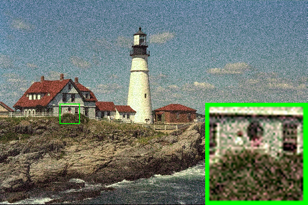
\includegraphics[width=1\textwidth]{comparea/resize_br_Noisy_nSig402030_kodim21.png}}
{\footnotesize (a) Noisy kodim21: 18.28dB }
\end{minipage}
\begin{minipage}[t]{0.195\textwidth}
\centering
\raisebox{-0.15cm}{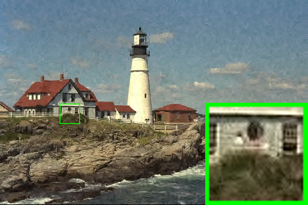
\includegraphics[width=1\textwidth]{comparea/resize_br_CBM3D_nSig402030_kodim21.png}}
{\footnotesize (b) CBM3D \cite{cbm3d}: 26.54dB}
\end{minipage}
\begin{minipage}[t]{0.195\textwidth}
\centering
\raisebox{-0.15cm}{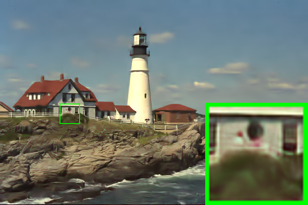
\includegraphics[width=1\textwidth]{comparea/resize_br_MLP_nSig402030_kodim21.png}}
{\footnotesize (c) MLP \cite{mlp}: 27.53dB}
\end{minipage}
\begin{minipage}[t]{0.195\textwidth}
\centering
\raisebox{-0.15cm}{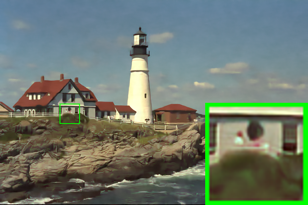
\includegraphics[width=1\textwidth]{comparea/resize_br_TNRD_nSig402030_kodim21.png}}
{\footnotesize (d) TNRD \cite{chen2015learning}: 27.60dB }
\end{minipage}
\centering
\begin{minipage}[t]{0.195\textwidth}
\raisebox{-0.15cm}{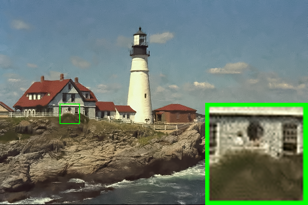
\includegraphics[width=1\textwidth]{comparea/resize_br_NC_nSig402030_kodim21.png}}
{\footnotesize (e) NC \cite{noiseclinic,ncwebsite}: 26.48dB  } 
\end{minipage}
}\vspace{-3mm}
\subfigure{
\begin{minipage}[t]{0.195\textwidth}
\centering
\raisebox{-0.15cm}{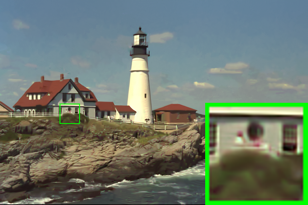
\includegraphics[width=1\textwidth]{comparea/resize_br_WNNMCW_nSig402030_kodim21.png}}
{\footnotesize (f) WNNM0: 27.80dB  }
\end{minipage}
\begin{minipage}[t]{0.195\textwidth}
\centering
\raisebox{-0.15cm}{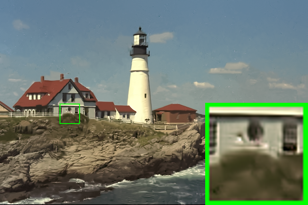
\includegraphics[width=1\textwidth]{comparea/resize_br_WNNMJ_nSig402030_kodim21.png}}
{\footnotesize (g) WNNM1: 27.75dB  }
\end{minipage}
\begin{minipage}[t]{0.195\textwidth}
\centering
\raisebox{-0.15cm}{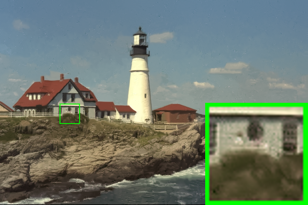
\includegraphics[width=1\textwidth]{comparea/resize_br_WNNM_ADMM_nSig402030_kodim21.png}}
{\footnotesize (h) WNNM2: 27.12dB }
\end{minipage}
\begin{minipage}[t]{0.195\textwidth}
\centering
\raisebox{-0.15cm}{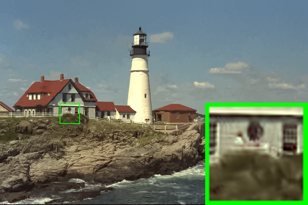
\includegraphics[width=1\textwidth]{comparea/resize_br_CWNNM_ADMM_nSig402030_kodim21.png}}
{\footnotesize (i) MC-WNNM: \textbf{28.34}dB}
\end{minipage}
\begin{minipage}[t]{0.195\textwidth}
\centering
\raisebox{-0.15cm}{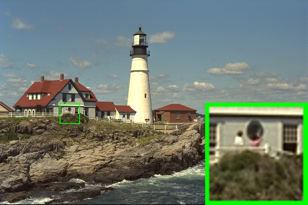
\includegraphics[width=1\textwidth]{comparea/resize_br_kodim21.png}}
{\footnotesize (j) Clean kodim21}
\end{minipage}
}\vspace{-0.5mm}
\caption{Denoised images of different methods on the image ``kodim21'' degraded by AWGN with different standard derivations of $\sigma_{r}=40, \sigma_{g}=20, \sigma_{b}=30$ on R, G, B channels, respectively. The images are better to be zoomed in on screen.}
\label{f1}
\vspace{-3mm}
\end{figure*}



\section{More visual comparisons of denoised images by different methods on the real noisy images of the dataset \cite{ncwebsite}}

In this section, we give more comparisons of the state-of-the-art denoising methods on the dataset \cite{ncwebsite}.\ The real noisy images in dataset \cite{ncwebsite} have no ``ground truth" images and hence we only compare the visual quality of the denoised images by different methods.\ As can be seen from Figures \ref{fig1}-\ref{fig4}, our proposed method performs better than the competing methods.

%------------------------------------------------------------------------------------
\begin{figure}
\centering
\subfigure{
\begin{minipage}[t]{0.2\textwidth}
\centering
\raisebox{-0.15cm}{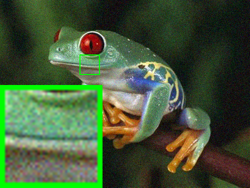
\includegraphics[width=1\textwidth]{imagessupp/resize_frog_noisy.png}}
{\footnotesize (a) Noisy \cite{ncwebsite}   }
\end{minipage}
\begin{minipage}[t]{0.2\textwidth}
\centering
\raisebox{-0.15cm}{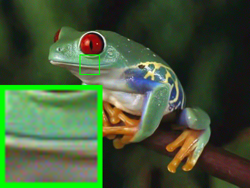
\includegraphics[width=1\textwidth]{imagessupp/resize_frog_cbm3d.png}}
{\footnotesize (b) CBM3D \cite{cbm3d}  }
\end{minipage}
\begin{minipage}[t]{0.2\textwidth}
\centering
\raisebox{-0.15cm}{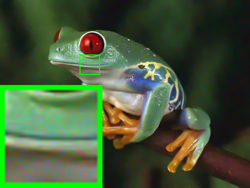
\includegraphics[width=1\textwidth]{imagessupp/resize_frog_mlp.png}}
{\footnotesize (c) MLP \cite{mlp}  }
\end{minipage}
\begin{minipage}[t]{0.2\textwidth}
\centering
\raisebox{-0.15cm}{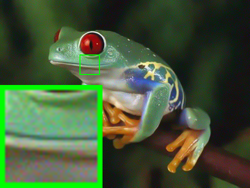
\includegraphics[width=1\textwidth]{imagessupp/resize_frog_tnrd.png}}
{\footnotesize (d) TNRD \cite{chen2015learning}}
\end{minipage}
\begin{minipage}[t]{0.2\textwidth}
\centering
\raisebox{-0.15cm}{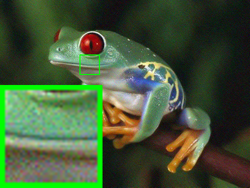
\includegraphics[width=1\textwidth]{imagessupp/resize_frog_ni.png}}
{\footnotesize (e) NI \cite{neatimage}  }
\end{minipage}
}\vspace{-3mm}
\subfigure{
\begin{minipage}[t]{0.2\textwidth}
\centering
\raisebox{-0.15cm}{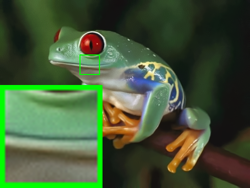
\includegraphics[width=1\textwidth]{imagessupp/resize_frog_nc.png}}
{\footnotesize (f) NC \cite{noiseclinic,ncwebsite}   }
\end{minipage}
\begin{minipage}[t]{0.2\textwidth}
\centering
\raisebox{-0.15cm}{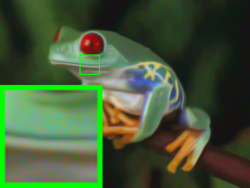
\includegraphics[width=1\textwidth]{imagessupp/resize_frog_wnnm.png}}
{\footnotesize (g) WNNM-1 \cite{wnnm}   }
\end{minipage}
\begin{minipage}[t]{0.2\textwidth}
\centering
\raisebox{-0.15cm}{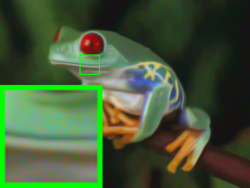
\includegraphics[width=1\textwidth]{imagessupp/resize_frog_wnnm.png}}
{\footnotesize (h) WNNM-2 \cite{wnnm}   }
\end{minipage}
\begin{minipage}[t]{0.2\textwidth}
\centering
\raisebox{-0.15cm}{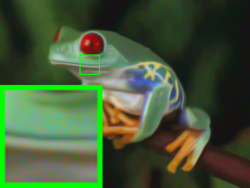
\includegraphics[width=1\textwidth]{imagessupp/resize_frog_wnnm.png}}
{\footnotesize (i) WNNM-3 \cite{wnnm}   }
\end{minipage}
\begin{minipage}[t]{0.2\textwidth}
\centering
\raisebox{-0.15cm}{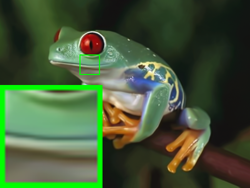
\includegraphics[width=1\textwidth]{imagessupp/resize_frog_ours.png}}
{\footnotesize (j) MC-WNNM  }
\end{minipage}
}
\vspace{-2mm}
\caption{Denoised images of the real noisy image ``Frog'' \cite{ncwebsite} by different methods.\ The images are better to be zoomed in on screen.}
\label{f3}
\end{figure}


%------------------------------------------------------------------------------------
\begin{figure}
\centering
\subfigure{
\begin{minipage}[t]{0.2\textwidth}
\centering
\raisebox{-0.15cm}{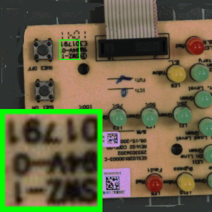
\includegraphics[width=1\textwidth]{imagessupp/resize_br_Noisy_circuit.png}}
{\footnotesize (a) Noisy \cite{ncwebsite}   }
\end{minipage}
\begin{minipage}[t]{0.2\textwidth}
\centering
\raisebox{-0.15cm}{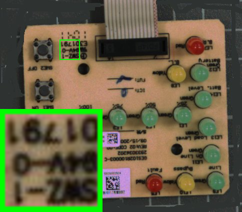
\includegraphics[width=1\textwidth]{imagessupp/resize_br_BM3D_circuit.png}}
{\footnotesize (b) CBM3D \cite{cbm3d}  }
\end{minipage}
\begin{minipage}[t]{0.2\textwidth}
\centering
\raisebox{-0.15cm}{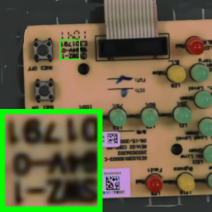
\includegraphics[width=1\textwidth]{imagessupp/resize_br_MLP_circuit.png}}
{\footnotesize (c) MLP \cite{mlp}  }
\end{minipage}
\begin{minipage}[t]{0.2\textwidth}
\centering
\raisebox{-0.15cm}{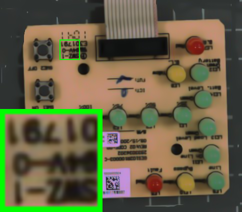
\includegraphics[width=1\textwidth]{imagessupp/resize_br_TRD_circuit.png}}
{\footnotesize (d) TNRD \cite{chen2015learning}}
\end{minipage}
\begin{minipage}[t]{0.2\textwidth}
\centering
\raisebox{-0.15cm}{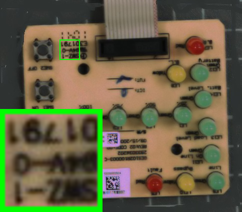
\includegraphics[width=1\textwidth]{imagessupp/resize_br_NI_circuit.png}}
{\footnotesize (e) NI \cite{neatimage}  }
\end{minipage}
}\vspace{-3mm}
\subfigure{
\begin{minipage}[t]{0.2\textwidth}
\centering
\raisebox{-0.15cm}{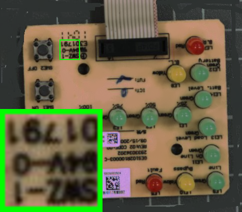
\includegraphics[width=1\textwidth]{imagessupp/resize_br_NC_circuit.png}}
{\footnotesize (f) NC \cite{noiseclinic,ncwebsite}   }
\end{minipage}
\begin{minipage}[t]{0.2\textwidth}
\centering
\raisebox{-0.15cm}{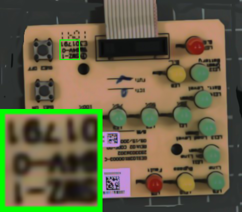
\includegraphics[width=1\textwidth]{imagessupp/resize_br_WNNM_circuit.png}}
{\footnotesize (g) WNNM-1 \cite{wnnm}   }
\end{minipage}
\begin{minipage}[t]{0.2\textwidth}
\centering
\raisebox{-0.15cm}{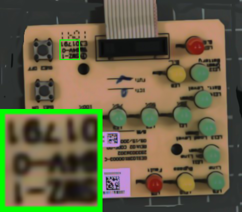
\includegraphics[width=1\textwidth]{imagessupp/resize_br_WNNM_circuit.png}}
{\footnotesize (h) WNNM-2 \cite{wnnm}   }
\end{minipage}
\begin{minipage}[t]{0.2\textwidth}
\centering
\raisebox{-0.15cm}{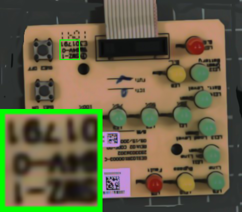
\includegraphics[width=1\textwidth]{imagessupp/resize_br_WNNM_circuit.png}}
{\footnotesize (i) WNNM-3 \cite{wnnm}   }
\end{minipage}
\begin{minipage}[t]{0.2\textwidth}
\centering
\raisebox{-0.15cm}{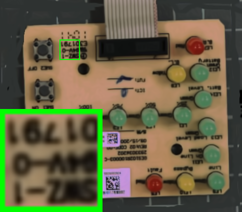
\includegraphics[width=1\textwidth]{imagessupp/resize_br_Guided_circuit.png}}
{\footnotesize (j) MC-WNNM  }
\end{minipage}
}
\vspace{-2mm}
\caption{Denoised images of the real noisy image ``Circuit'' \cite{ncwebsite} by different methods.\ The images are better to be zoomed in on screen.}
\label{f3}
\end{figure}


%------------------------------------------------------------------------------------
\begin{figure}
\centering
\subfigure{
\begin{minipage}[t]{0.2\textwidth}
\centering
\raisebox{-0.15cm}{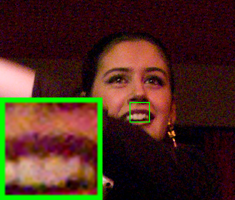
\includegraphics[width=1\textwidth]{imagessupp/resize_br_Noisy_woman.png}}
{\footnotesize (a) Noisy \cite{ncwebsite}   }
\end{minipage}
\begin{minipage}[t]{0.2\textwidth}
\centering
\raisebox{-0.15cm}{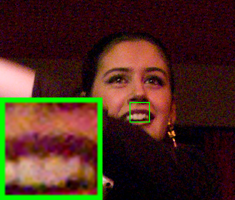
\includegraphics[width=1\textwidth]{imagessupp/resize_br_BM3D_woman.png}}
{\footnotesize (b) CBM3D \cite{cbm3d}  }
\end{minipage}
\begin{minipage}[t]{0.2\textwidth}
\centering
\raisebox{-0.15cm}{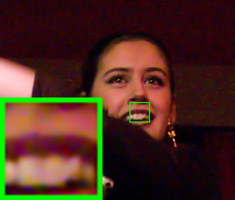
\includegraphics[width=1\textwidth]{imagessupp/resize_br_MLP_woman.png}}
{\footnotesize (c) MLP \cite{mlp}  }
\end{minipage}
\begin{minipage}[t]{0.2\textwidth}
\centering
\raisebox{-0.15cm}{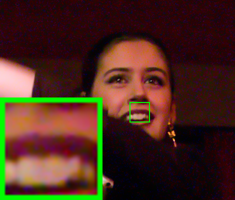
\includegraphics[width=1\textwidth]{imagessupp/resize_br_TRD_woman.png}}
{\footnotesize (d) TNRD \cite{chen2015learning}}
\end{minipage}
\begin{minipage}[t]{0.2\textwidth}
\centering
\raisebox{-0.15cm}{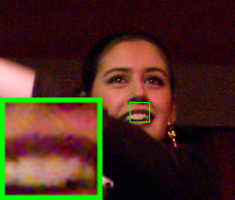
\includegraphics[width=1\textwidth]{imagessupp/resize_br_NI_woman.png}}
{\footnotesize (e) NI \cite{neatimage}  }
\end{minipage}
}\vspace{-3mm}
\subfigure{
\begin{minipage}[t]{0.2\textwidth}
\centering
\raisebox{-0.15cm}{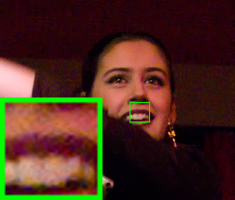
\includegraphics[width=1\textwidth]{imagessupp/resize_br_NC_woman.png}}
{\footnotesize (f) NC \cite{noiseclinic,ncwebsite}   }
\end{minipage}
\begin{minipage}[t]{0.2\textwidth}
\centering
\raisebox{-0.15cm}{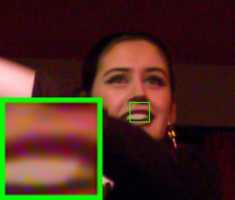
\includegraphics[width=1\textwidth]{imagessupp/resize_br_WNNM_woman.png}}
{\footnotesize (g) WNNM-1 \cite{wnnm}   }
\end{minipage}
\begin{minipage}[t]{0.2\textwidth}
\centering
\raisebox{-0.15cm}{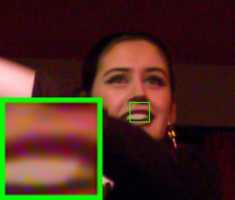
\includegraphics[width=1\textwidth]{imagessupp/resize_br_WNNM_woman.png}}
{\footnotesize (h) WNNM-2 \cite{wnnm}   }
\end{minipage}
\begin{minipage}[t]{0.2\textwidth}
\centering
\raisebox{-0.15cm}{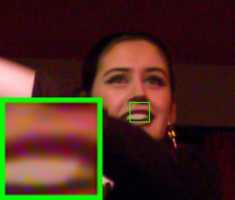
\includegraphics[width=1\textwidth]{imagessupp/resize_br_WNNM_woman.png}}
{\footnotesize (i) WNNM-3 \cite{wnnm}   }
\end{minipage}
\begin{minipage}[t]{0.2\textwidth}
\centering
\raisebox{-0.15cm}{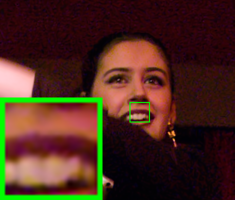
\includegraphics[width=1\textwidth]{imagessupp/resize_br_Guided_woman.png}}
{\footnotesize (j) MC-WNNM  }
\end{minipage}
}
\vspace{-2mm}
\caption{Denoised images of the real noisy image ``Woman'' \cite{ncwebsite} by different methods.\ The images are better to be zoomed in on screen.}
\label{f3}
\vspace{-2mm}
\end{figure}



%------------------------------------------------------------------------------------
\begin{figure}
\centering
\subfigure{
\begin{minipage}[t]{0.2\textwidth}
\centering
\raisebox{-0.15cm}{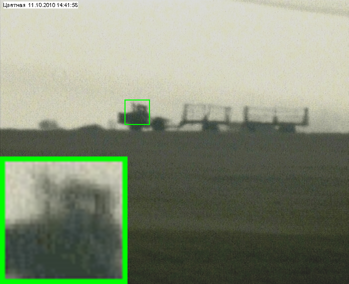
\includegraphics[width=1\textwidth]{imagessupp/resize_br_Noisy_vehicle.png}}
{\footnotesize (a) Noisy \cite{ncwebsite}   }
\end{minipage}
\begin{minipage}[t]{0.2\textwidth}
\centering
\raisebox{-0.15cm}{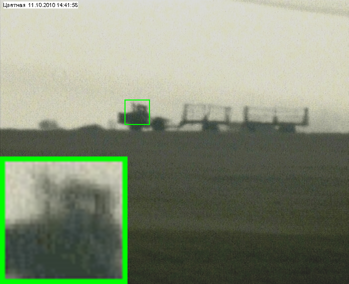
\includegraphics[width=1\textwidth]{imagessupp/resize_br_BM3D_vehicle.png}}
{\footnotesize (b) CBM3D \cite{cbm3d}  }
\end{minipage}
\begin{minipage}[t]{0.2\textwidth}
\centering
\raisebox{-0.15cm}{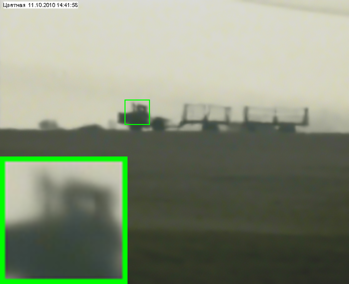
\includegraphics[width=1\textwidth]{imagessupp/resize_br_MLP_vehicle.png}}
{\footnotesize (c) MLP \cite{mlp}  }
\end{minipage}
\begin{minipage}[t]{0.2\textwidth}
\centering
\raisebox{-0.15cm}{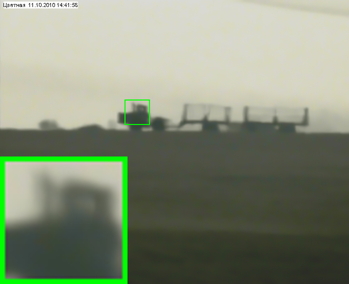
\includegraphics[width=1\textwidth]{imagessupp/resize_br_TRD_vehicle.png}}
{\footnotesize (d) TNRD \cite{chen2015learning}}
\end{minipage}
\begin{minipage}[t]{0.2\textwidth}
\centering
\raisebox{-0.15cm}{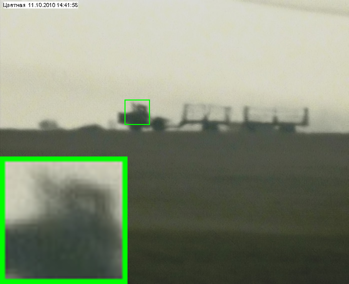
\includegraphics[width=1\textwidth]{imagessupp/resize_br_NI_vehicle.png}}
{\footnotesize (e) NI \cite{neatimage}  }
\end{minipage}
}\vspace{-3mm}
\subfigure{
\begin{minipage}[t]{0.2\textwidth}
\centering
\raisebox{-0.15cm}{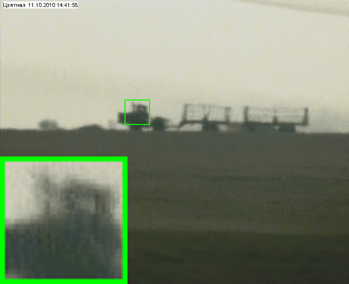
\includegraphics[width=1\textwidth]{imagessupp/resize_br_NC_vehicle.png}}
{\footnotesize (f) NC \cite{noiseclinic,ncwebsite}   }
\end{minipage}
\begin{minipage}[t]{0.2\textwidth}
\centering
\raisebox{-0.15cm}{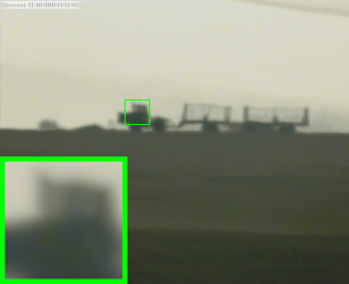
\includegraphics[width=1\textwidth]{imagessupp/resize_br_WNNM_vehicle.png}}
{\footnotesize (g) WNNM-1 \cite{wnnm}   }
\end{minipage}
\begin{minipage}[t]{0.2\textwidth}
\centering
\raisebox{-0.15cm}{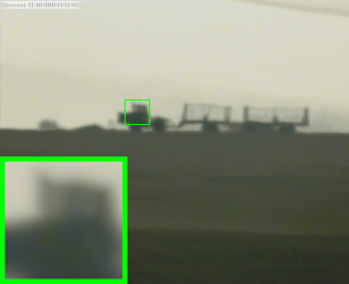
\includegraphics[width=1\textwidth]{imagessupp/resize_br_WNNM_vehicle.png}}
{\footnotesize (h) WNNM-2 \cite{wnnm}   }
\end{minipage}
\begin{minipage}[t]{0.2\textwidth}
\centering
\raisebox{-0.15cm}{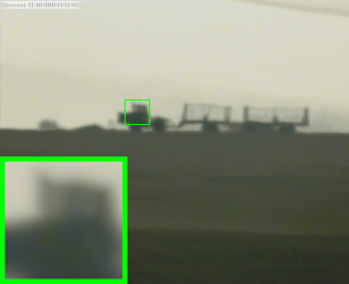
\includegraphics[width=1\textwidth]{imagessupp/resize_br_WNNM_vehicle.png}}
{\footnotesize (i) WNNM-3 \cite{wnnm}   }
\end{minipage}
\begin{minipage}[t]{0.2\textwidth}
\centering
\raisebox{-0.15cm}{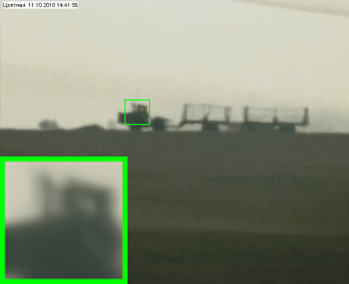
\includegraphics[width=1\textwidth]{imagessupp/resize_br_Guided_vehicle.png}}
{\footnotesize (j) MC-WNNM  }
\end{minipage}
}
\vspace{-2mm}
\caption{Denoised images of the real noisy image ``Vehicle'' \cite{ncwebsite} by different methods.\ The images are better to be zoomed in on screen.}
\label{f3}
\vspace{-2mm}
\end{figure}





\section{More visual comparisons of denoised images by different methods on the real noisy images of the dataset \cite{crosschannel2016}}

In this section, we provide more comparisons of the proposed method with the state-of-the-art denoising methods on the 15 cropped real noisy images used in \cite{crosschannel2016}.\ In this dataset, each scene was shot 500 times under the same camera and camera setting.\ The mean image of the 500 shots is roughly taken as the ``ground truth", with which the PSNR can be computed.\ As can be seen from Figures \ref{fig5}-\ref{fig9}, in most cases, our proposed method achieves better performance than the the competing methods.\ This validates the effectiveness of our proposed external prior guided internal prior learning framework for real noisy image denoising.


%------------------------------------------------------------------------------------
\begin{figure}\vspace{3mm}
\centering
\subfigure{
\begin{minipage}[t]{0.195\textwidth}
\centering
\raisebox{-0.15cm}{\includegraphics[width=1\textwidth]{imagessupp/resize_resize_br_Noisy_5dmark3_iso3200_2_real.png}}
{\footnotesize (a) Noisy  \cite{crosschannel2016}: 33.88dB }
\end{minipage}
\begin{minipage}[t]{0.195\textwidth}
\centering
\raisebox{-0.15cm}{\includegraphics[width=1\textwidth]{imagessupp/resize_resize_br_CBM3D_5dmark3_iso3200_2_real.png}}
{\footnotesize (b) CBM3D \cite{bm3d,cbm3d}: 33.91dB}
\end{minipage}
\centering
\begin{minipage}[t]{0.195\textwidth}
\raisebox{-0.15cm}{\includegraphics[width=1\textwidth]{imagessupp/resize_resize_br_TRD_5dmark3_iso3200_2_real.png}}
{\footnotesize (c) TNRD \cite{chen2015learning}: 34.33dB  } 
\end{minipage}
\begin{minipage}[t]{0.195\textwidth}
\centering
\raisebox{-0.15cm}{\includegraphics[width=1\textwidth]{imagessupp/resize_resize_br_NI_5dmark3_iso3200_2_real.png}}
{\footnotesize (d) NI \cite{neatimage}: 34.87dB  }
\end{minipage}
\begin{minipage}[t]{0.195\textwidth}
\centering
\raisebox{-0.15cm}{\includegraphics[width=1\textwidth]{imagessupp/resize_resize_br_NC_5dmark3_iso3200_2_real.png}}
{\footnotesize (e) NC \cite{ncwebsite,noiseclinic}: 35.69dB  }
\end{minipage}
}\vspace{-2mm}
\subfigure{
\begin{minipage}[t]{0.195\textwidth}
\centering
\raisebox{-0.15cm}{\includegraphics[width=1\textwidth]{imagessupp/resize_resize_br_CCNoise_5dmark3_iso3200_2.png}}
{\footnotesize (f) CC \cite{crosschannel2016}: 35.37dB }
\end{minipage}
\begin{minipage}[t]{0.195\textwidth}
\centering
\raisebox{-0.15cm}{\includegraphics[width=1\textwidth]{imagessupp/resize_resize_br_WNNM_5dmark3_iso3200_2_real.png}}
{\footnotesize (g) WNNM-2 \cite{wnnm}: 33.88dB}
\end{minipage}
\begin{minipage}[t]{0.195\textwidth}
\centering
\raisebox{-0.15cm}{\includegraphics[width=1\textwidth]{imagessupp/resize_resize_br_WNNM_5dmark3_iso3200_2_real.png}}
{\footnotesize (h) WNNM-3 \cite{wnnm}: 33.88dB}
\end{minipage}
\begin{minipage}[t]{0.195\textwidth}
\centering
\raisebox{-0.15cm}{\includegraphics[width=1\textwidth]{imagessupp/resize_resize_br_Guided_5dmark3_iso3200_2_real.png}}
{\footnotesize (i) Ours: \textbf{37.05}dB}
\end{minipage}
\begin{minipage}[t]{0.195\textwidth}
\centering
\raisebox{-0.15cm}{\includegraphics[width=1\textwidth]{imagessupp/resize_resize_br_Mean_5dmark3_iso3200_2_real.png}}
{\footnotesize (j) Mean Image \cite{crosschannel2016}}
\end{minipage}
}
\caption{Denoised images of a region cropped from the real noisy image ``Canon 5D Mark 3 ISO 3200 2" \cite{crosschannel2016} by different methods. The images are better to be zoomed in on screen.}
\label{fig5}
\end{figure}


%------------------------------------------------------------------------------------
\begin{figure}\vspace{3mm}
\centering
\subfigure{
\begin{minipage}[t]{0.195\textwidth}
\centering
\raisebox{-0.15cm}{\includegraphics[width=1\textwidth]{imagessupp/resize_resize_br_Noisy_d600_iso3200_2_real.png}}
{\footnotesize (a) Noisy  \cite{crosschannel2016}: 33.88dB }
\end{minipage}
\begin{minipage}[t]{0.195\textwidth}
\centering
\raisebox{-0.15cm}{\includegraphics[width=1\textwidth]{imagessupp/resize_resize_br_CBM3D_d600_iso3200_2_real.png}}
{\footnotesize (b) CBM3D \cite{bm3d,cbm3d}: 33.91dB}
\end{minipage}
\centering
\begin{minipage}[t]{0.195\textwidth}
\raisebox{-0.15cm}{\includegraphics[width=1\textwidth]{imagessupp/resize_resize_br_TRD_d600_iso3200_2_real.png}}
{\footnotesize (c) TNRD \cite{chen2015learning}: 34.33dB  } 
\end{minipage}
\begin{minipage}[t]{0.195\textwidth}
\centering
\raisebox{-0.15cm}{\includegraphics[width=1\textwidth]{imagessupp/resize_resize_br_NI_d600_iso3200_2_real.png}}
{\footnotesize (d) NI \cite{neatimage}: 34.87dB  }
\end{minipage}
\begin{minipage}[t]{0.195\textwidth}
\centering
\raisebox{-0.15cm}{\includegraphics[width=1\textwidth]{imagessupp/resize_resize_br_NC_d600_iso3200_2_real.png}}
{\footnotesize (e) NC \cite{ncwebsite,noiseclinic}: 35.69dB  }
\end{minipage}
}\vspace{-2mm}
\subfigure{
\begin{minipage}[t]{0.195\textwidth}
\centering
\raisebox{-0.15cm}{\includegraphics[width=1\textwidth]{imagessupp/resize_resize_br_CCNoise_d600_iso3200_2.png}}
{\footnotesize (f) CC \cite{crosschannel2016}: 35.37dB }
\end{minipage}
\begin{minipage}[t]{0.195\textwidth}
\centering
\raisebox{-0.15cm}{\includegraphics[width=1\textwidth]{imagessupp/resize_resize_br_WNNM_d600_iso3200_2_real.png}}
{\footnotesize (g) WNNM-2 \cite{wnnm}: 33.88dB}
\end{minipage}
\begin{minipage}[t]{0.195\textwidth}
\centering
\raisebox{-0.15cm}{\includegraphics[width=1\textwidth]{imagessupp/resize_resize_br_WNNM_d600_iso3200_2_real.png}}
{\footnotesize (h) WNNM-3 \cite{wnnm}: 33.88dB}
\end{minipage}
\begin{minipage}[t]{0.195\textwidth}
\centering
\raisebox{-0.15cm}{\includegraphics[width=1\textwidth]{imagessupp/resize_resize_br_Guided_d600_iso3200_2_real.png}}
{\footnotesize (i) Ours: \textbf{37.05}dB}
\end{minipage}
\begin{minipage}[t]{0.195\textwidth}
\centering
\raisebox{-0.15cm}{\includegraphics[width=1\textwidth]{imagessupp/resize_resize_br_Mean_d600_iso3200_2_real.png}}
{\footnotesize (j) Mean Image \cite{crosschannel2016}}
\end{minipage}
}
\caption{Denoised images of a region cropped from the real noisy image ``Nikon D600 ISO 1600 2" \cite{crosschannel2016} by different methods. The images are better to be zoomed in on screen.}
\label{fig5}
\end{figure}




%------------------------------------------------------------------------------------
\begin{figure}\vspace{3mm}
\centering
\subfigure{
\begin{minipage}[t]{0.195\textwidth}
\centering
\raisebox{-0.15cm}{\includegraphics[width=1\textwidth]{imagessupp/resize_resize_br_Noisy_d800_iso3200_2_real.png}}
{\footnotesize (a) Noisy  \cite{crosschannel2016}: 33.88dB }
\end{minipage}
\begin{minipage}[t]{0.195\textwidth}
\centering
\raisebox{-0.15cm}{\includegraphics[width=1\textwidth]{imagessupp/resize_resize_br_CBM3D_d800_iso3200_2_real.png}}
{\footnotesize (b) CBM3D \cite{bm3d,cbm3d}: 33.91dB}
\end{minipage}
\centering
\begin{minipage}[t]{0.195\textwidth}
\raisebox{-0.15cm}{\includegraphics[width=1\textwidth]{imagessupp/resize_resize_br_TRD_d800_iso3200_2_real.png}}
{\footnotesize (c) TNRD \cite{chen2015learning}: 34.33dB  } 
\end{minipage}
\begin{minipage}[t]{0.195\textwidth}
\centering
\raisebox{-0.15cm}{\includegraphics[width=1\textwidth]{imagessupp/resize_resize_br_NI_d800_iso3200_2_real.png}}
{\footnotesize (d) NI \cite{neatimage}: 34.87dB  }
\end{minipage}
\begin{minipage}[t]{0.195\textwidth}
\centering
\raisebox{-0.15cm}{\includegraphics[width=1\textwidth]{imagessupp/resize_resize_br_NC_d800_iso3200_2_real.png}}
{\footnotesize (e) NC \cite{ncwebsite,noiseclinic}: 35.69dB  }
\end{minipage}
}\vspace{-2mm}
\subfigure{
\begin{minipage}[t]{0.195\textwidth}
\centering
\raisebox{-0.15cm}{\includegraphics[width=1\textwidth]{imagessupp/resize_resize_br_CCNoise_d800_iso3200_2.png}}
{\footnotesize (f) CC \cite{crosschannel2016}: 35.37dB }
\end{minipage}
\begin{minipage}[t]{0.195\textwidth}
\centering
\raisebox{-0.15cm}{\includegraphics[width=1\textwidth]{imagessupp/resize_resize_br_WNNM_d800_iso3200_2_real.png}}
{\footnotesize (g) WNNM-2 \cite{wnnm}: 33.88dB}
\end{minipage}
\begin{minipage}[t]{0.195\textwidth}
\centering
\raisebox{-0.15cm}{\includegraphics[width=1\textwidth]{imagessupp/resize_resize_br_WNNM_d800_iso3200_2_real.png}}
{\footnotesize (h) WNNM-3 \cite{wnnm}: 33.88dB}
\end{minipage}
\begin{minipage}[t]{0.195\textwidth}
\centering
\raisebox{-0.15cm}{\includegraphics[width=1\textwidth]{imagessupp/resize_resize_br_Guided_d800_iso3200_2_real.png}}
{\footnotesize (i) Ours: \textbf{37.05}dB}
\end{minipage}
\begin{minipage}[t]{0.195\textwidth}
\centering
\raisebox{-0.15cm}{\includegraphics[width=1\textwidth]{imagessupp/resize_resize_br_Mean_d800_iso3200_2_real.png}}
{\footnotesize (j) Mean Image \cite{crosschannel2016}}
\end{minipage}
}
\caption{Denoised images of a region cropped from the real noisy image ``Nikon D800 ISO 1600 2" \cite{crosschannel2016} by different methods. The images are better to be zoomed in on screen.}
\label{fig5}
\end{figure}



%------------------------------------------------------------------------------------
\begin{figure}\vspace{1mm}
\centering
\subfigure{
\begin{minipage}[t]{0.195\textwidth}
\centering
\raisebox{-0.15cm}{\includegraphics[width=1\textwidth]{imagessupp/resize_resize_br_Noisy_d800_iso6400_2_real.png}}
{\footnotesize (a) Noisy  \cite{crosschannel2016}: 32.89dB }
\end{minipage}
\begin{minipage}[t]{0.195\textwidth}
\centering
\raisebox{-0.15cm}{\includegraphics[width=1\textwidth]{imagessupp/resize_resize_br_CBM3D_d800_iso6400_2_real.png}}
{\footnotesize (b) CBM3D \cite{bm3d,cbm3d}: 32.91dB}
\end{minipage}
\begin{minipage}[t]{0.195\textwidth}
\centering
\raisebox{-0.15cm}{\includegraphics[width=1\textwidth]{imagessupp/resize_resize_br_WNNM_d800_iso6400_2_real.png}}
{\footnotesize (c) WNNM \cite{wnnm}: 32.94dB}
\end{minipage}
\begin{minipage}[t]{0.195\textwidth}
\centering
\raisebox{-0.15cm}{\includegraphics[width=1\textwidth]{imagessupp/resize_resize_br_MLP_d800_iso6400_2_real.png}}
{\footnotesize (d) MLP \cite{mlp}: 34.87dB } 
\end{minipage}
\centering
\begin{minipage}[t]{0.195\textwidth}
\raisebox{-0.15cm}{\includegraphics[width=1\textwidth]{imagessupp/resize_resize_br_TRD_d800_iso6400_2_real.png}}
{\footnotesize (e) TNRD \cite{chen2015learning}: 35.74dB  } 
\end{minipage}
}\vspace{-2mm}
\subfigure{
\begin{minipage}[t]{0.195\textwidth}
\centering
\raisebox{-0.15cm}{\includegraphics[width=1\textwidth]{imagessupp/resize_resize_br_NI_d800_iso6400_2_real.png}}
{\footnotesize (f) NI \cite{neatimage}: 35.09dB  }
\end{minipage}
\begin{minipage}[t]{0.195\textwidth}
\centering
\raisebox{-0.15cm}{\includegraphics[width=1\textwidth]{imagessupp/resize_resize_br_NC_d800_iso6400_2_real.png}}
{\footnotesize (g) NC \cite{ncwebsite,noiseclinic}: 35.72dB  }
\end{minipage}
\begin{minipage}[t]{0.195\textwidth}
\centering
\raisebox{-0.15cm}{\includegraphics[width=1\textwidth]{imagessupp/resize_resize_br_CCNoise_d800_iso6400_2.png}}
{\footnotesize (h) CC \cite{crosschannel2016}: 36.75dB }
\end{minipage}
\begin{minipage}[t]{0.195\textwidth}
\centering
\raisebox{-0.15cm}{\includegraphics[width=1\textwidth]{imagessupp/resize_resize_br_Guided_d800_iso6400_2_real.png}}
{\footnotesize (i) Ours: \textbf{37.07}dB}
\end{minipage}
\begin{minipage}[t]{0.195\textwidth}
\centering
\raisebox{-0.15cm}{\includegraphics[width=1\textwidth]{imagessupp/resize_resize_br_Mean_d800_iso6400_2_real.png}}
{\footnotesize (j) Mean Image \cite{crosschannel2016}}
\end{minipage}
}
\caption{Denoised images of a region cropped from the real noisy image ``Nikon D800 ISO 6400 2" \cite{crosschannel2016} by different methods. The images are better to be zoomed in on screen.}
\label{fig8}
\end{figure}


{
\small
\bibliographystyle{unsrt}
\bibliography{egbib}
}

\end{document}